\subsection{Misalignment of lenslet couple antenna systematic}

\paragraph{Description:}
With lenslet couple antenna technology, there is a possibility that lenslets will not be aligned with an antenna. This can occur from each individual pixel or entire wafer slipped from each other. For a case of  slipped in each individual pixel, this will be a random direction in entire wafer. For a case of entire of wafer, this can cause on how good we clamp between each wafers or thermal contraction between the wafer holder and the wafer. This scenario will be more likely to create systematic pointing error. 

\paragraph{Plan to model and/or measure:}
We can create a model in HFSS to simulate the effect to beam parameters from misalignment from lenslet couple antenna. After that we can use ray tracing program such as Zemax estimate how much of this contribute to overall pointing error on sky.

\paragraph{Uncertainty/Range:}
We can minimize an uncertainty from this by know all the possibilities that can cause a wafer slipped e.g. the thermal contraction from the wafer holder and wafer, or vibration from outside. Range of the uncertainty also vary by size of lenslets and antenna. In PB2 case, we set the tolerance level at 20 $\mu m$.

\paragraph{Parameterization:}
This is a result from HFSS that we simulated for PB2. This showed a linear relationship between the pointing error and the distance of lenslets and antenna. In the simulation also showed the direction of pointing offset is a same direction of wafer slipped. 
  
\begin{figure}
\centering
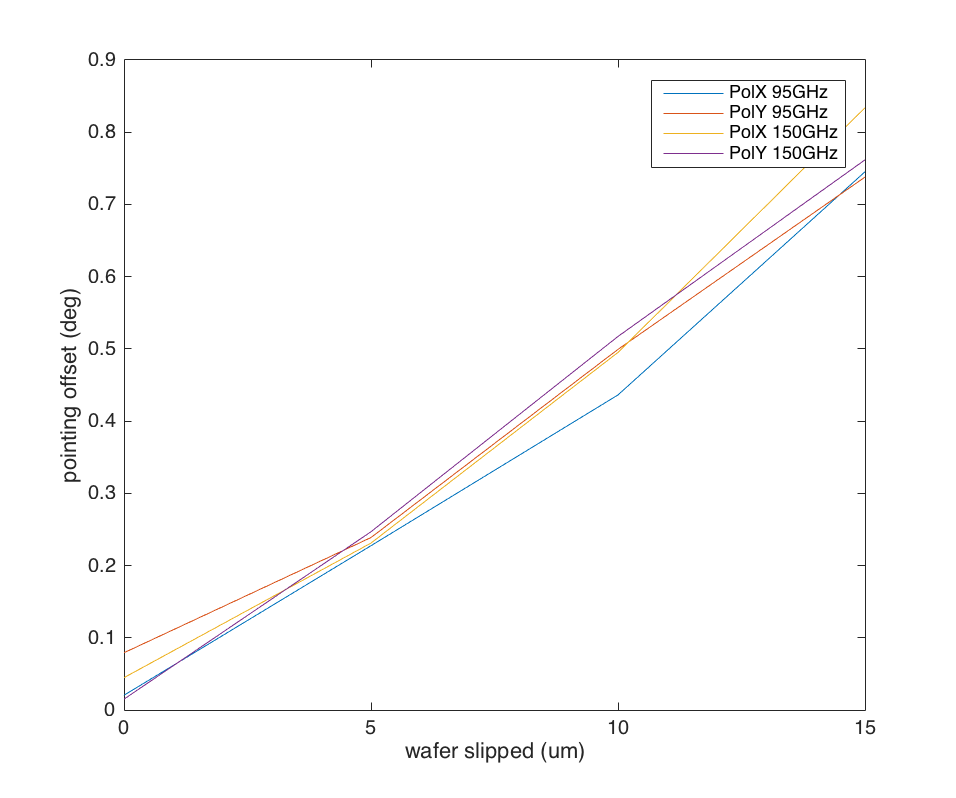
\includegraphics[width=3.25in]{figures/pointingOffset_waferslipped.png}
\caption{plot pointing error vs an offset between sinuous antenna and lenslet }
\label{poitingoffsetFromWaferslipped}
\end{figure}
